\documentclass[12pt,a4paper]{article}
\usepackage[utf8]{inputenc}
\usepackage[T1]{fontenc}
\usepackage[francais]{babel}
\usepackage{amsmath,empheq}
\usepackage{amsfonts}
\usepackage{amssymb}
\usepackage{graphicx}
\usepackage[top=2.00cm]{geometry}
\usepackage{titlesec}
\usepackage{multicol}
\usepackage{tikz,tkz-tab}
%%modif des titres de section diminuer la taille
\graphicspath{{images/}}
\renewcommand{\thesection}{\Roman{section}}
\titleformat{\section}
{\normalfont\bfseries\Large\scshape}{\thesection}{1em}{}
\titleformat{\subsection}
{\normalfont\bfseries\large}{\thesubsection}{1em}{}
\makeatletter
\def\@maketitle{
	\begin{center}
	% NoLogo
	%	\vspace*{+2cm}
	
	%	Corner Logo
	%	\begin{flushright}
	%		
\includegraphics[width=40mm]{logo_corner}\\[4ex]
	%	\end{flushright}
	
	%	Top Logo
		
\includegraphics[scale=0.3]{logo_top}
			
				{\LARGE \@title }\\[4ex]
				{\large \@author}\\[4ex]
				{\large \@date}\\[8ex]
		\rule{\linewidth}{0.4pt}
	\end{center}
}
\makeatletter

\author{CHARNAY Valentin, FINOT Sylvain}
\title{Compte rendu de TP :\\ \scshape Optique Géométrique}

\date{4 février 2017}
\begin{document}
\maketitle
\section{Mesures de distances focales}
\subsection{Méthode de Silbermann}
On considère le montage suivant :\\
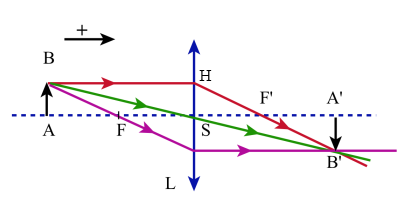
\includegraphics[scale=4]{montageSilberman}\\
On pose : 
$$
\begin{aligned}
\gamma = \dfrac{\overline{A'B'}}{\overline{AB}} ,\quad y=\overline{AA'},\quad p=\overline{SA},\quad p'=\overline{SA'},\quad \phi=\overline{SF'}=\overline{FS}
\end{aligned}
$$
Montrons que $y=-\phi\dfrac{{(\gamma-1)}^2}{\gamma}$:
\begin{multicols}{2}
	\begingroup
	\addtolength{\jot}{1em}
	\noindent
	\begin{align*}
	\dfrac{1}{p'}-\dfrac{1}{p}&=\dfrac{1}{\phi}\quad \text{relation de conjugaison}\\
\iff	p'&=\dfrac{p\phi}{p+\phi}\\
	p'-p &= \dfrac{p\phi}{p+\phi}-p\\
	y &= \dfrac{p\phi-p(p+\phi)}{p+\phi}\\
	y&=-\dfrac{p^2}{p+\phi}
	\end{align*}
	\endgroup
	\setlength\columnseprule{0.4pt}
	\vfill
	\columnbreak
	D'autre part en appliquant le théorème de Thalès aux triangle SHF' et F'A'B':
	\begingroup
	\addtolength{\jot}{1em}
	\noindent
	\begin{align*}
	\gamma&\equiv\dfrac{\overline{A'B'}}{\overline{AB}} = \dfrac{\overline{A'B'}}{\overline{SH}}\\
	&=\dfrac{\overline{A'F'}}{\overline{SF'}}\\
	&=\dfrac{\overline{A'S}+\overline{SF'}}{\overline{SF'}}\\
	&=\dfrac{-p'}{\phi}+1\\
	\iff p' &= -\phi(\gamma-1)
	\end{align*}
	\endgroup
\end{multicols}
\vspace*{+1em}
De plus on sait que : $\dfrac {\overline {AB}} {p}=\dfrac {\overline {A'B'}} {p'}\implies\dfrac{p'}{p}=\gamma$, ainsi :
\begin{empheq}[left=\empheqlbrace]{align}
	y&=-\dfrac{p^2}{p+\phi}\\
	p' &= -\phi(\gamma-1)\\
	\dfrac{p'}{p}&=\gamma
\end{empheq}

\end{document}
